\section{Spezielle Operationsverstärker}

\subsection{Unkompensierte Opamps}

\begin{minipage}{9cm}
	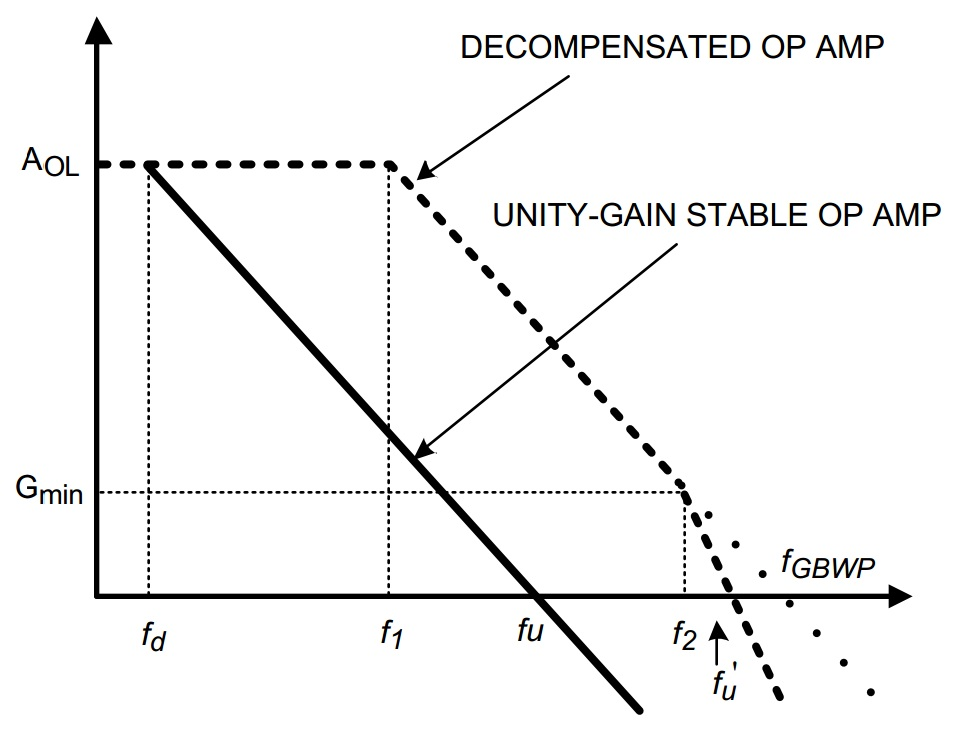
\includegraphics[width=7cm]{images/op_uncomp.jpg}
\end{minipage}
\begin{minipage}{-9cm+\linewidth}
	Während normale Opamps bis zu Gain $\pm 1$ stabil sind, benötigen
	unkompensierte Opamps einen minimalen Gain $G_{min}$ (z.B. $10$) um
	stabil zu sein. \\
	
	Die Pole werden durch die fehlende Kompensation höher liegen, womit
	ein höheres Gain-Bandwith-Product erreicht wird (z.B. 88 MHz statt 17 MHz)
\end{minipage}


\subsection{Current Feedback Amplifier (CFA)}
VFA und CFA werden gleich beschaltet, mit einem CFA sind jedoch höhere
Bandbreiten bei höherer Verstärkung möglich. CFA werden daher für schnelle
Treiber eingesetzt, und oft in Bipolar-Technologie aufgebaut. Der Nachteil
des CFA ist die grössere Offset-Spannung. \\

\begin{tabularx}{\linewidth}{p{3cm}XX}
	&\textbf{Voltage Feedback Opamp (VFA)} & \textbf{Current Feedback Opamp (CFA)} \\
	\hline
	& 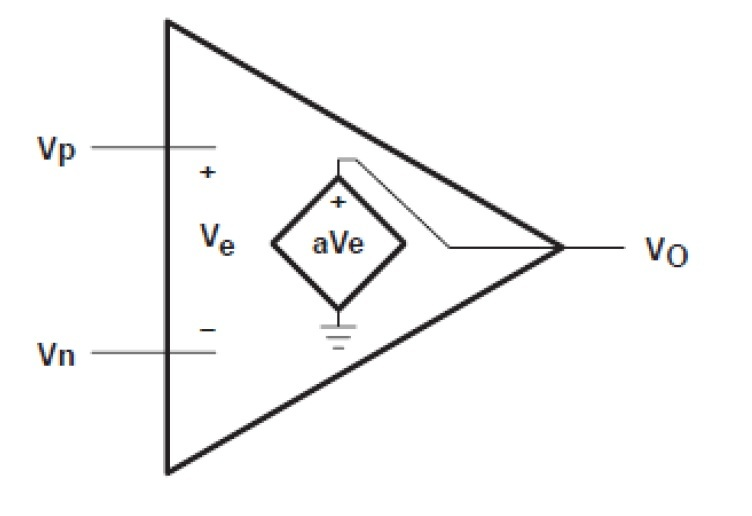
\includegraphics[width=3cm]{images/op_vfa.jpg} & 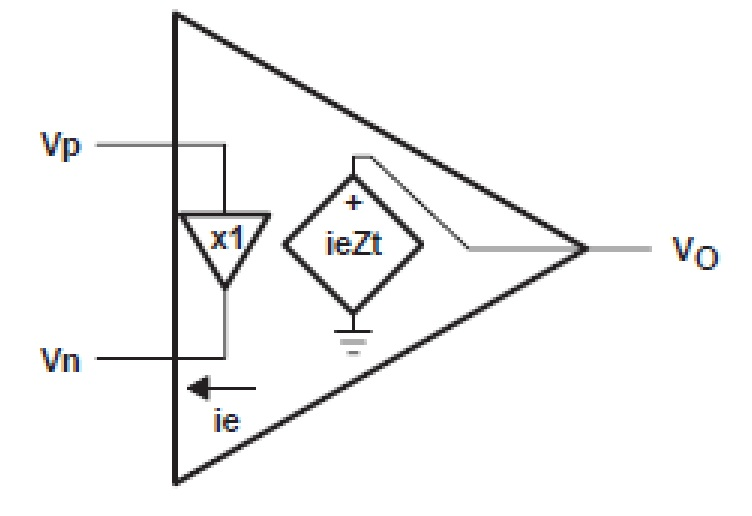
\includegraphics[width=3cm]{images/op_cfa.jpg} \\
	Eigenschaften: & Hochohmige Eingänge \newline hohe Spannungsverstärkung $A$ & Buffer von $V_p$ nach $V_n$ \newline $V_p$: hochohmiger Eingang, $V_n$: niederohmiger Ausgang \\
	Invertierender Verstärker & $b = \frac{R_1}{R_1 + R_2}$ \newline $\frac{V_o}{V_i} = \frac{1}{b} \frac{1}{1+\frac{1}{a b}}$ \newline Error term $\frac{1}{ab}$ ist abhängig vom Gain. & $b = \frac{R_1}{R_1 + R_2}$ \newline $\frac{V_o}{V_i} = \frac{1}{b} \frac{1}{1 + \frac{R_2}{Z_t}}$ \newline Error term $\frac{R_2}{Z_t}$ ist unabhängig von $R_1$ und damit vom Gain $1/b$. \\
	& $f_c = \frac{g_m}{2 \pi C_c} \frac{R_1}{R_1 + R_2}$ \newline grösserer Gain $\Rightarrow$ kleinere Bandbreite & $\frac{V_o}{V_i} \simeq \frac{R_1 + R_2}{R_1} \frac{1}{1 + j 2 \pi f R_2 C_c}$ \newline Bandbreite nur von $C_c$ und $R_2$ abhängig. \\
	\hline
\end{tabularx}


\subsection{Diamond Transistor}
Der Operational Transconductance Amplifier (OTA), Diamond Transistor oder
Voltage controlled current source, kann wie ein (fast) idealer Transistor
betrachtet werden. 

\begin{center}
	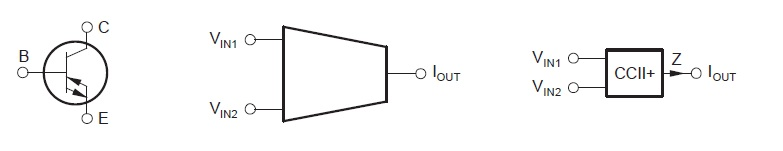
\includegraphics[width=12cm]{images/op_diamond}
\end{center}

\begin{tabular}{lllll}
	\textbf{NPN Transistor} & $V_{BE} \approx 0.7V$ & 
		$g_m$ nichtlinear $(g_m \sim I_C)$ & $I_C > 0$ & $I_E \approx-I_C$ \\
	\textbf{Diamond Transistor} & $V_{BE} = 0V$ & $I_C = g_m V_{BE}$ &
		$I_C$ positiv und negativ & $I_E = I_C$ \\
\end{tabular}

\subsection{gmC Filter}
\begin{multicols}{2}
	Für Transkonduktanz-Verstärker gilt:
	\begin{equation*}
		I_{\Out} = g_m \left( V_{\In 2} - V_{\In 1} \right)
	\end{equation*}
	
	$g_m$ wird durch den Bias-Strom eingestellt. 
	Damit sind Filter möglich, welche flexibel über $I_{\text{bias}}$ oder $U_{\text{bias}}$ eingestellt werden können. \\
	
	\paragraph{Integrator mit OTA}~\\
	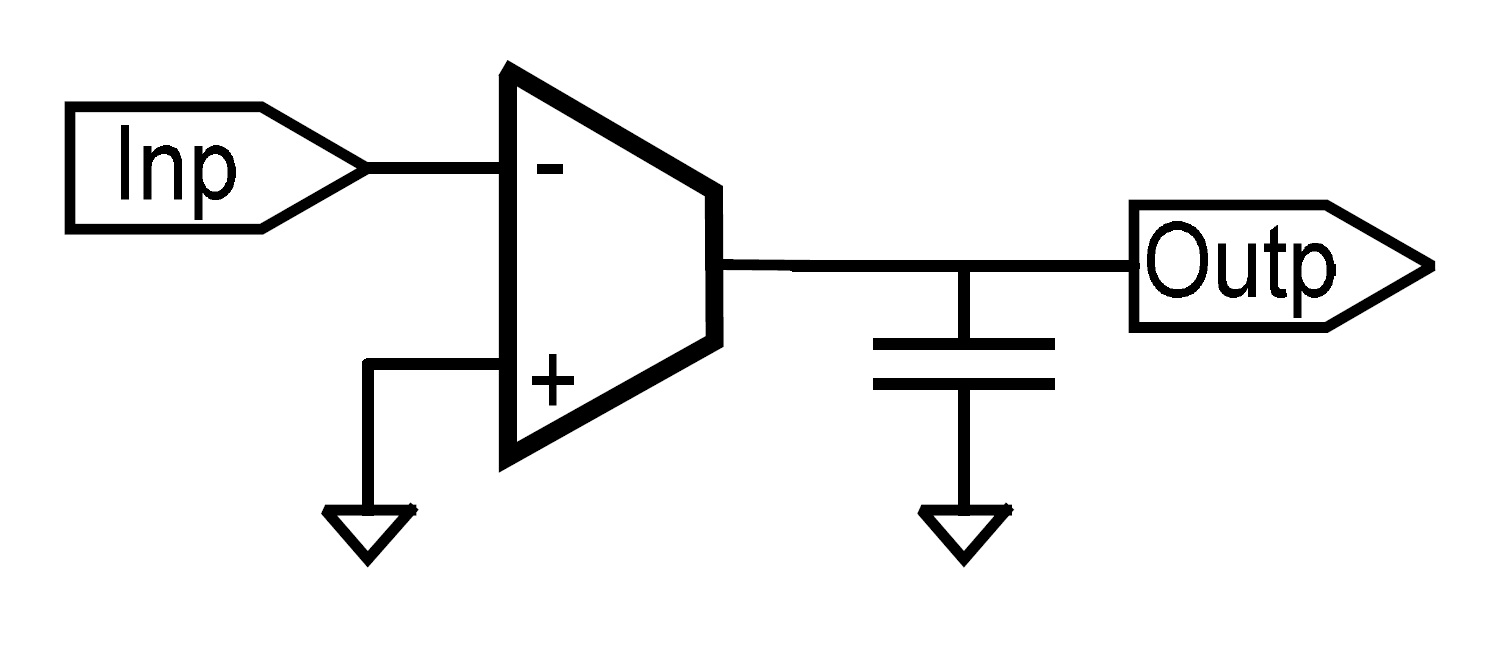
\includegraphics[width=5cm]{images/gmC_filter.jpg}

	\begin{align*}
		I_{\Out}(t) &= -g_m V_{\In} (t) \\
		V_{\Out}(t) &= \frac{-g_m}{C} \int V_{\In}(t) dt
	\end{align*}
\end{multicols}